\chapter{系统实现}

\newcommand{\chapterfiveplaceholder}[1]{%
\begin{center}
\fbox{\parbox[c][4.0cm][c]{0.82\textwidth}{\centering #1（占位）}}
\end{center}
\begin{center}
#1（占位）
\end{center}
}
\newcommand{\thesiscirclednum}[1]{\ding{\numexpr191+#1\relax}}
\newcommand{\thesisdescitem}[3]{%
\par\addvspace{0.55\baselineskip}%
\noindent\hspace*{2em}\thesiscirclednum{#1}\ #2\par
\vspace{0.1\baselineskip}%
\noindent\hspace*{2em}#3\par
}
\newcommand{\thesisparenitem}[3]{%
\par\addvspace{0.55\baselineskip}%
\noindent\hspace*{2em}（#1）\ #2\par
\vspace{0.1\baselineskip}%
\noindent\hspace*{2em}#3\par
}

\tikzset{
  chapterfivebox/.style={rectangle, draw, rounded corners=2pt, minimum width=3.7cm, minimum height=0.9cm, text centered, align=center},
  chapterfivedecision/.style={diamond, draw, minimum width=2.8cm, minimum height=1.0cm, text centered, aspect=2},
  chapterfivearrow/.style={->, >=Stealth, thick}
}

本章主要介绍系统的实际实现。前文已经完成需求分析和总体设计，这一章转向具体落地，重点说明后端、Web 前端和桌面端分别如何实现核心功能。本系统后端负责鉴权、消息存储、AI 调用和 Socket.IO 实时通信，前端负责聊天界面、状态同步、桌面端托盘和通知交互\cite{expressdocs2026,socketiodocs2026,electrondocs2026}。下面按后端、Web 前端和桌面端三个部分展开说明。

\section{后端实现}

\subsection{后端项目结构说明}

本系统后端由主入口文件统一完成服务启动和基础配置加载，具体业务再按职责拆分到路由、控制器、模型、Socket 事件、AI 代理和服务模块中。这样可以避免单个文件承担过多逻辑，也方便后续扩展接口、调整数据模型和排查实时通信问题。整体上，后端核心内容可以概括为配置层、路由层、控制器层、数据模型层、实时通信层以及 AI 服务与工具层。

\thesisparenitem{1}{\texttt{config}}{主要处理数据库连接和 OAuth 配置。MongoDB 连接在数据库配置文件中完成，Google、GitHub 登录策略则在第三方登陆中注册。}
\thesisparenitem{2}{\texttt{routes}}{负责把请求路径分配给不同业务模块。用户、私聊、聊天室、AI、收藏和上传接口都在这一层挂接。}
\thesisparenitem{3}{\texttt{controllers}}{负责具体业务逻辑。前端发起的登录、消息发送和历史记录读取等请求，最终都会在这一层完成处理。}
\thesisparenitem{4}{\texttt{models}}{对应 MongoDB 文档结构。系统把私聊消息和群聊消息分开建模，和前端界面的功能划分保持一致。}
\thesisparenitem{5}{\texttt{middlewares}}{中间件中中较关键的是验证模块，它负责 JWT 校验，用于控制受保护接口的访问。}
\thesisparenitem{6}{\texttt{sockets}}{负责 Socket.IO 事件。私聊、群聊、语音房间和代码协作分别独立放置，便于按功能定位实时通信问题。}
\thesisparenitem{7}{\texttt{agents}、\texttt{services} 和 \texttt{tools}}{一起组成 AI 能力。这一部分不是简单封装模型调用，而是实现了带有步骤编排的 Agent 结构。}

本项目设计的这套拆分方式已经能够覆盖当前聊天系统的核心需求。后续如果继续增加消息审核、AI 角色管理或者更细的权限控制，也可以沿着这套结构继续扩展，不会混淆旧代码。

\subsection{核心模块实现}

\subsubsection{用户模块}

本系统的用户模块支持邮箱密码登录、邮箱验证码登录、邮箱注册，以及 Google、GitHub 的 OAuth 登录。实现上，用户认证、路由分发和第三方登录配置分别落在对应模块中。登录成功以后，系统返回 JWT，前端再把 token 和用户信息保存到本地，并继续初始化 Socket 连接和在线状态\cite{oauthcn2024,oauthbcp2025}。

用户登录成功后，系统会统一生成带有效期的 JWT，并在响应中同时返回用户标识、昵称、邮箱与头像等基础资料，方便前端一次完成身份保持、用户信息回填和 Socket 初始化。

用户认证模块围绕统一身份体系展开。普通注册时，后端会先校验邮箱格式和密码强度，再使用 \texttt{bcrypt} 对密码进行哈希；普通登录时，则根据邮箱查询用户并比对哈希结果，验证通过后再生成 token。验证码登录流程先通过邮件服务生成并暂存验证码，用户提交后再完成核验。OAuth 登录需要先从第三方平台获取用户资料，再根据第三方 ID 或邮箱匹配本地账户，未匹配到时自动创建新账户。该设计使不同登录方式可以共用同一套用户数据。

后端在 \texttt{/api/user/info} 用户信息接口中统一返回当前用户的基础信息。前端在登录完成后通过该接口补齐头像和邮箱，设置页修改资料后也会再次请求该接口；OAuth 回调完成后，前端同样会先读取当前用户信息，再决定后续页面跳转。因此，用户模块不仅承担登录和注册功能，也为其他页面提供统一的身份基础。

邮箱密码登录与 JWT 下发的相关实现见附录A。

\subsubsection{聊天模块}

本系统的聊天模块分成私聊和群聊两条主线。私聊围绕一对一消息收发与历史查询展开，群聊和技术聊天室则同时支持多人讨论、问题标记和协作交流。除最基础的文本消息外，系统还支持图片、文件、语音、代码片段、引用回复和问题标记。

群聊消息在进入数据库前会先补齐发送者昵称、头像、消息类型和引用信息等字段，写库完成后再更新房间活跃时间，并通过房间广播把完整消息对象同步给在线成员。

群聊消息发送时，后端会先确认房间是否存在以及当前用户是否为成员，再补齐发送者昵称和头像，最后将消息写入群消息集合。其中，群消息文档会冗余保存 \texttt{fromName} 和 \texttt{fromAvatar}，从而避免前端在加载历史消息时逐条查询用户表。私聊部分采用相近思路，但数据结构相对更简洁，核心字段主要包括 \texttt{from}、\texttt{to}、\texttt{content} 和 \texttt{isRead}。

从数据模型设计看，群聊并不等同于简单的多人私聊。群消息模型中额外定义了 \texttt{quotedMessage}、\texttt{isQuestion}、\texttt{questionStatus}、\texttt{isSolution}、\texttt{reactions} 等字段，用于对应前端的技术讨论功能。例如，用户在聊天室中标记问题、设置最佳答案或添加表情反应时，相关状态都会写入消息文档，而不是仅停留在界面层。这样一来，聊天室中的问题追踪与讨论辅助功能就有了明确的数据模型支撑。

私聊消息查询与发送、技术聊天室创建等相关实现分别见附录B与附录C。

\subsubsection{AI智能检索与流式交互（RAG \& SSE）}

本系统的 AI 模块将ai流式对话接口设计为结合 RAG 向量检索与 Server-Sent Events (SSE) 的流式处理接口。当用户在聊天室中发送带有 \texttt{@AI} 的问题时，系统不会直接把请求转发给模型，而是先整理当前房间的上下文，再调用模型生成回答\cite{qaoverview2025,ragllmsurvey2024,ragsurveycn2025}。

\begin{figure}[H]
\centering
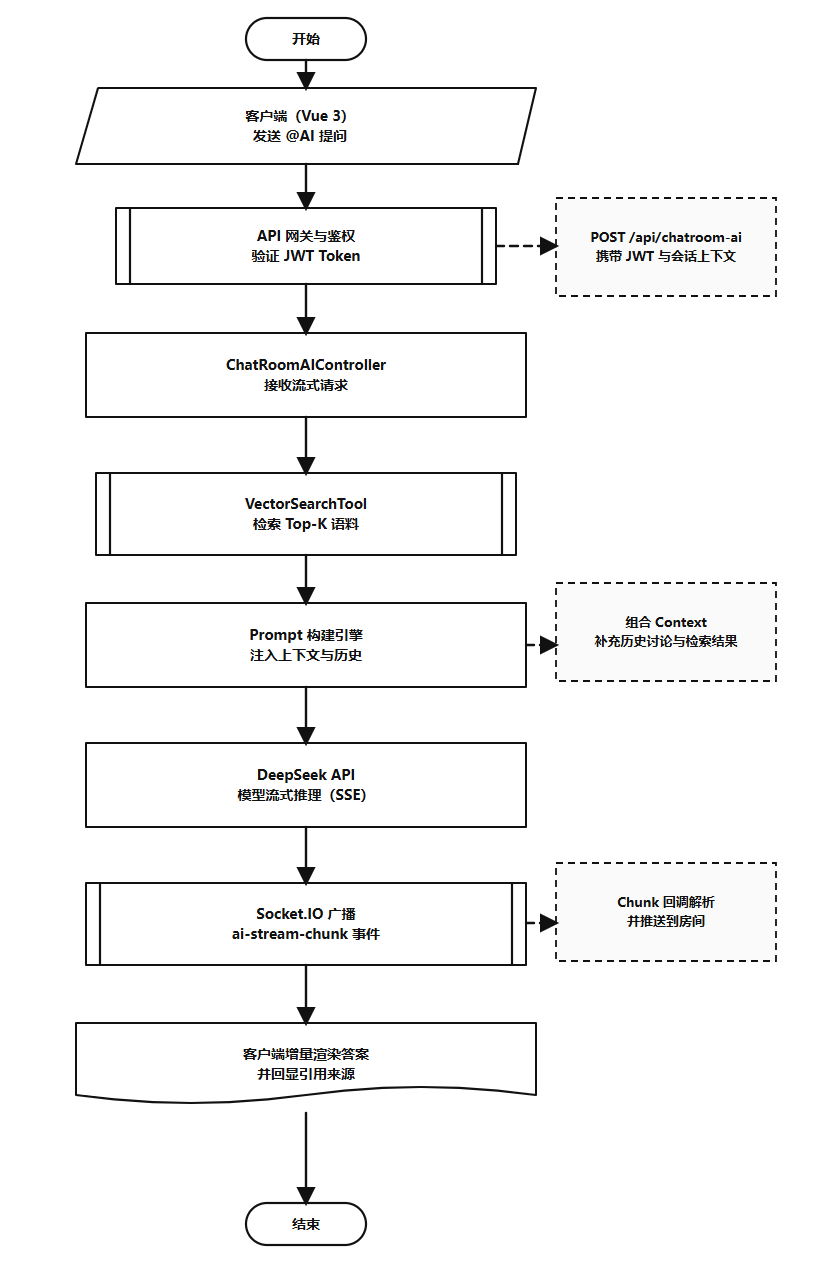
\includegraphics[width=0.94\textwidth,height=0.58\textheight,keepaspectratio]{img/图5_1.png}
\caption{RAG智能流式问答核心处理流}
\label{fig:5-20}
\end{figure}

如图~\ref{fig:5-20}所示，系统先通过向量检索工具在 MongoDB 历史集合中检索 Top-5 相关聊天记录，并将结果整理进 Prompt，再向模型发起流式请求。

在拼装好检索上下文后，后端会发起流式模型请求，并把增量内容同时写回 SSE 响应和ai流式广播事件。这样一来，提问者和同房间成员都能实时看到回答逐段生成。

该接口把 HTTP 的 SSE 响应和 WebSocket 房间广播结合在一起。提问者通过长连接逐步接收生成内容，同一房间内的其他成员则通过监听ai流式事件获取增量结果。对于响应耗时较长的大语言模型请求，这种分块返回机制能够缩短首字节等待时间（TTFB），也更适合多人协作场景\cite{deepseekrag2026}。

聊天室 AI 流式回复与结果落库的相关实现见附录D。

\subsubsection{WebSocket模块}

本系统通过 WebSocket 承载私聊通知、房间广播、在线状态同步以及协作类实时事件。实现上，私聊事件和房间级事件分开组织，语音交流和代码协作也单独拆分，从而避免所有实时逻辑堆叠在同一处\cite{socketiodocs2026,imsecurity2024}。

WebSocket 层分别维护“用户到 socket 集合”和“房间到在线用户集合”的映射关系，在广播消息前先完成连接归属和用户去重，再回推在线人数与消息增量。

WebSocket 层没有直接使用 \texttt{socket.id} 作为用户标识，而是建立了两层映射关系。私聊部分的用户表维护一个用户对应一组 socket 连接，从而支持同一账号在多个窗口同时登录；群聊部分的 \texttt{roomUsers} 记录“某个房间内在线的 userId 集合”，因此在线人数统计会按用户去重，避免同一用户的多窗口连接被重复计算。

此外，本系统没有将所有实时事件集中在同一个入口处理。私聊消息、群消息、语音连麦和代码协作分别独立实现，这样既便于后续按模块维护，也有助于在出现问题时快速定位具体事件链路。

房间在线状态维护与群消息广播的相关实现见附录E。

\subsubsection{数据模型与辅助模块}

后端在核心聊天主链路之外，还提供了上传、收藏、问题追踪、代码片段保存、消息索引和链接预览等辅助能力。这些模块共同支撑了技术交流场景下的信息保存、检索和回看需求。

群消息模型除了发送者、内容和时间等基础字段外，还扩展了引用回复、问题标记、表情反应和附件信息等结构，为收藏、历史检索和 AI 分析提供了统一的数据基础。

这一部分不仅补充了前端可见的功能入口，也补充了对应的数据结构。例如，引用回复、问题标记和表情反应都直接定义在消息模型中；收藏模块会保存消息快照，因此即使原消息被删除，收藏内容仍可回读；上传模块先保存文件，再将文件地址写回消息记录，使图片、语音和文件能够在历史消息中继续访问。此外，系统还通过消息向量化索引和RAG服务对文本消息进行向量化索引，为后续 AI 检索提供支持\cite{mongodbdocs2026,llmplatform2024}。

收藏数据写入与来源回读的相关实现见附录F。

\subsubsection{聊天室洞察与智能话题聚类分析}

对于一个活跃的技术交流平台，仅靠被动等待用户输入还不够，系统还需要具备整理房间讨论情况的能力。为此，本系统设计了 \texttt{getRoomInsights} 接口，用来汇总房间消息的整体状态。

\begin{figure}[H]
\centering
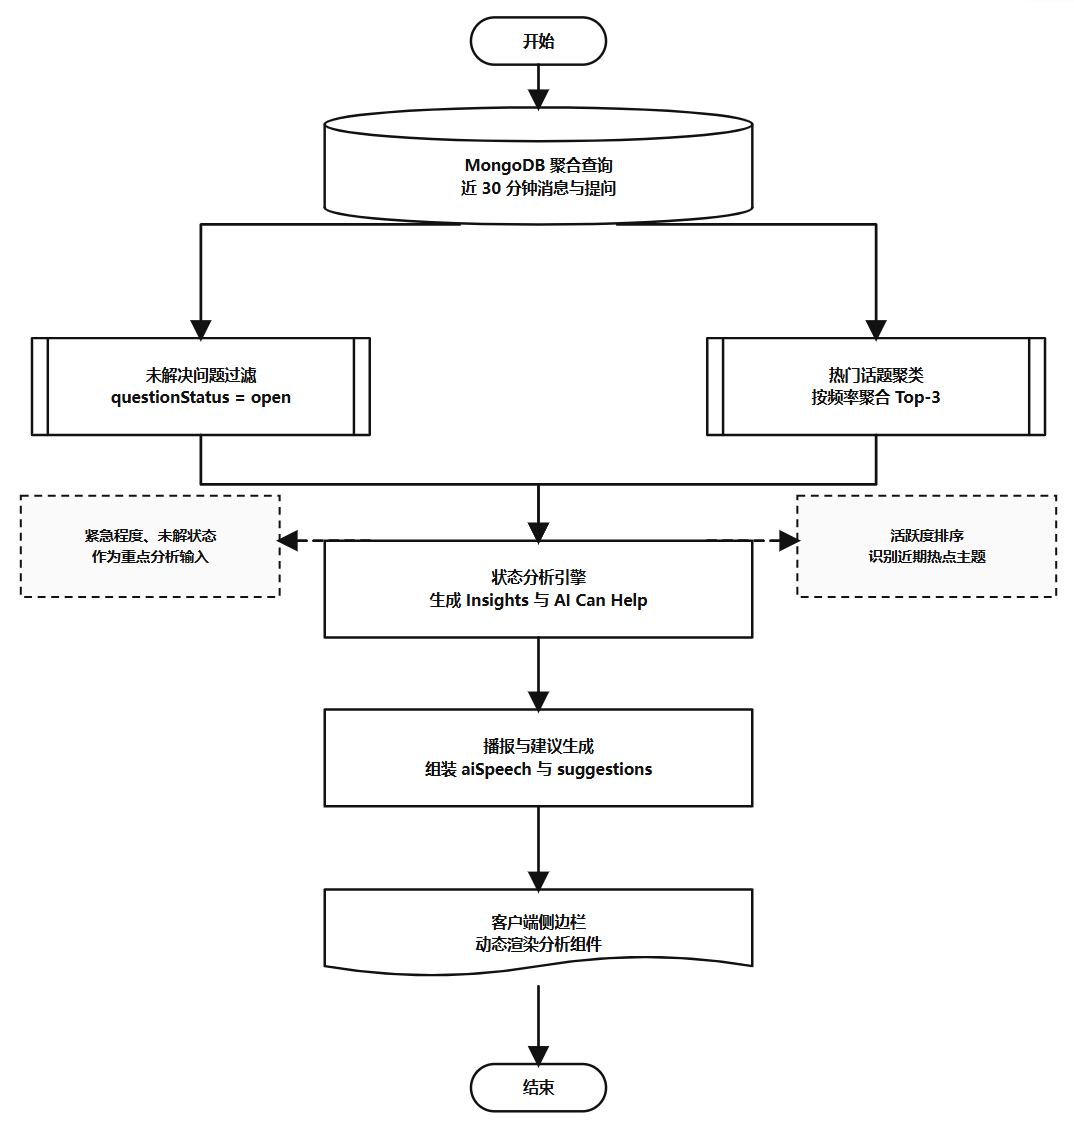
\includegraphics[width=0.94\textwidth,height=0.54\textheight,keepaspectratio]{img/图5_2.png}
\caption{聊天室实时洞察与状态分析流}
\label{fig:5-21}
\end{figure}

如图~\ref{fig:5-21}所示，该功能主要依靠 MongoDB 文档数据库的聚合能力完成统计，并未额外引入复杂的机器学习流程。

洞察模块先筛出未解决问题，再基于最近消息构建话题映射，统计讨论热度与参与者范围，最后把聚合结果整理成结构化的 \texttt{insights} 报告供前端展示。

系统先按时间窗口整理最近 30 分钟的数据，再利用 Map/Set 结构完成遍历和去重，最后把结果整理成扁平化的 \texttt{insights} 评估报告，并生成 \texttt{aiSpeech} 回传给前端展示。这样一来，用户可以直接看到哪些问题还没有解决、哪些话题仍在持续讨论，而不必完全依赖手动翻看消息记录。


\subsection{接口设计}

结合后端主入口、路由分发和具体业务处理逻辑，本系统常用接口可以分成普通 REST 接口、AI 接口和 WebSocket 通信接口三类。这里不把所有接口都逐一展开，而是挑出最能代表系统实现特点的几组进行说明，并结合表中内容概括每一类接口承担的职责。

\thesisparenitem{1}{普通 REST 接口设计}{这一部分主要包含用户认证、用户资料读取、私聊历史查询以及聊天室消息写入等标准 HTTP 请求接口。它们的共同特点是一次请求、一次返回，重点解决身份校验、数据持久化和列表查询等基础业务问题，是前端大多数页面能够正常工作的前提。普通 REST 接口的代表性设计如表~\ref{tab:5-1}所示。}

\begin{table}[!tbp]
\centering
\caption{普通 REST 接口设计}
\label{tab:5-1}
\small
\renewcommand{\arraystretch}{1.15}
\setlength{\tabcolsep}{0.7ex}
\begin{tabular}{M{0.16\textwidth}M{0.22\textwidth}M{0.10\textwidth}p{0.23\textwidth}p{0.19\textwidth}}
\toprule
\textbf{接口名称} & \textbf{请求路径} & \textbf{请求方式} & \textbf{参数说明} & \textbf{返回示例} \\
\midrule
发送验证码 & \parbox[t]{0.20\textwidth}{\raggedright \texttt{/api/user/}\\\texttt{send-verification}} & POST & \texttt{email}、\texttt{type} & 返回提示信息 \\
邮箱密码登录 & \texttt{/api/user/login-email} & POST & \texttt{email}、\texttt{password} & 返回 \texttt{token} 与用户信息 \\
获取当前用户信息 & \texttt{/api/user/info} & GET & Bearer Token & 返回 \texttt{user} 对象 \\
获取私聊消息 & \parbox[t]{0.20\textwidth}{\raggedright \texttt{/api/chat/}\\\texttt{messages/:id}} & GET & 路径参数为对方用户 ID & 返回消息数组 \\
发送群聊消息 & \parbox[t]{0.20\textwidth}{\raggedright \texttt{/room/:roomId/}\\\texttt{messages}} & POST & \texttt{content}、\texttt{messageType}、\texttt{quotedMessage} 等 & 返回消息对象 \\
\bottomrule
\end{tabular}
\end{table}

\noindent 表~\ref{tab:5-1}所列接口主要承担数据写入和稳定读取的任务。其中，登录、发送验证码和获取当前用户信息属于用户域接口，私聊消息读取和聊天室消息发送则属于会话域接口。这类接口并不追求长连接式的实时推送，而是强调参数明确、返回结构稳定和便于前后端分层调试。

\thesisparenitem{2}{AI 接口设计}{AI 接口主要服务于智能问答、文本解释和聊天总结等增强功能。与普通业务接口相比，它们通常需要拼接上下文、调用检索服务并进一步请求大语言模型，因此返回结果中不仅包含答案正文，还可能包含来源信息、置信度或结构化摘要内容。AI 接口的代表性设计如表~\ref{tab:5-2}所示。}

\begin{table}[!tbp]
\centering
\caption{AI 接口设计}
\label{tab:5-2}
\small
\renewcommand{\arraystretch}{1.15}
\setlength{\tabcolsep}{0.7ex}
\begin{tabular}{M{0.16\textwidth}M{0.22\textwidth}M{0.10\textwidth}p{0.23\textwidth}p{0.19\textwidth}}
\toprule
\textbf{接口名称} & \textbf{请求路径} & \textbf{请求方式} & \textbf{参数说明} & \textbf{返回示例} \\
\midrule
侧边栏智能问答 & \texttt{/api/agent/chat} & POST & \texttt{question}、\texttt{chatType}、\texttt{sessionId} 等 & 返回答案、来源和置信度 \\
会话总结 & \texttt{/api/agent/summarize} & POST & \texttt{chatType}、\texttt{targetId/roomId}、\texttt{timeRange} & 返回结构化总结 \\
划词解释 & \texttt{/api/agent/explain} & POST & \texttt{text}、\texttt{isFollowUp} & 返回解释文本 \\
聊天室流式问答 & \parbox[t]{0.20\textwidth}{\raggedright \texttt{/api/chatroom-ai/}\\\texttt{ask-stream}} & POST & \texttt{roomId}、\texttt{question}、\texttt{useRAG} & 以 SSE 分块返回结果 \\
\bottomrule
\end{tabular}
\end{table}

\noindent 表~\ref{tab:5-2}反映出，AI 接口并不是单一的一条问答接口，而是根据使用场景分成了侧边栏智能问答、会话总结、划词解释和聊天室流式问答四种类型。这样的拆分有助于把单人查询、多轮解释”和多人协作中的 AI 区分开来，也方便前端在不同页面里选择更合适的交互方式。

\thesisparenitem{3}{WebSocket 通信接口设计}{WebSocket 部分主要用于处理用户上线注册、私聊消息通知、加入聊天室、群消息广播以及 AI 流式输出同步等事件。它与前两类接口最大的不同，在于它强调服务端主动推送和多端实时同步，更适合承载聊天系统里的在线状态与增量消息场景。WebSocket 通信接口的代表性设计如表~\ref{tab:5-3}所示。}

\begin{table}[!tbp]
\centering
\caption{WebSocket 通信接口设计}
\label{tab:5-3}
\small
\renewcommand{\arraystretch}{1.15}
\setlength{\tabcolsep}{0.7ex}
\begin{tabular}{M{0.15\textwidth}M{0.20\textwidth}M{0.10\textwidth}p{0.24\textwidth}p{0.20\textwidth}}
\toprule
\textbf{接口名称} & \textbf{通信标识} & \textbf{触发方式} & \textbf{参数说明} & \textbf{返回示例} \\
\midrule
用户上线注册 & \texttt{login} & client emit & \texttt{userId} & 服务端登记在线状态并回推列表 \\
私聊消息通知 & \texttt{private-message} & 双向 & \texttt{from}、\texttt{to}、\texttt{content} 等 & 实时推送私聊消息 \\
加入聊天室 & \texttt{join-group} & client emit & \texttt{roomId}、\texttt{userId} & 触发在线人数和成员广播 \\
群消息广播 & \texttt{group-message} & 双向 & \texttt{roomId}、\texttt{content}、\texttt{fromName} 等 & 房间成员收到完整消息对象 \\
AI 增量输出 &ai流式& server emit & \texttt{roomId}、\texttt{content}、\texttt{isComplete} & 前端逐段渲染 AI 回答 \\
\bottomrule
\end{tabular}
\end{table}

\noindent 表~\ref{tab:5-3}反映出系统实时通信层的核心职责，即把“谁上线了”“谁加入了房间”“哪条消息需要立即同步给谁”这些高频事件从普通 HTTP 请求中拆出来单独处理。尤其是 \texttt{group-message} 与ai流式这类事件，直接决定了聊天室消息和 AI 回答能否在界面上即时呈现。

\FloatBarrier

\subsection{示例数据}

为了说明接口返回内容，下面给出两个更贴近实际格式的示例。字段名与系统实际返回结构保持一致，只对 token 和部分 ID 做了简化。

\thesisparenitem{1}{示例 1：邮箱密码登录接口返回}{返回体通常包含 \texttt{message}、\texttt{token} 和 \texttt{user} 三部分，其中 \texttt{user} 内含用户 ID、昵称、邮箱与头像地址，足以支撑前端完成登录后的首轮渲染。}

\thesisparenitem{2}{示例 2：智能问答接口返回}{返回体会以 \texttt{success} 标记请求结果，并在 \texttt{data} 中给出回答正文、来源片段、置信度、是否使用上下文以及检索条数等信息，用于前端展示答案与解释其生成依据。}

\subsection{通信机制说明}

\subsubsection{HTTP 通信流程}

普通业务请求大多遵循同一条链路：前端通过 Axios 发起请求，并在请求头中附带 token；服务端经过认证模块完成鉴权后，再进入具体业务处理；随后由数据模型读写 MongoDB，并将 \texttt{user}、消息记录等结果返回给前端。登录、获取当前用户信息、拉取历史消息、上传文件和创建聊天室等操作基本都按这一流程完成\cite{expressdocs2026,mongodbdocs2026}。

\subsubsection{WebSocket 实时通信流程}

实时通信与 HTTP 在系统中承担不同职责。HTTP 主要负责数据写入与读取，Socket.IO 则负责将状态变化和消息增量及时同步给在线成员。私聊发送时，前端通常先通过 REST 接口写库，再发送 \texttt{private-message} 通知对方刷新；群聊发送时，客户端完成消息提交后，由服务端主动广播 \texttt{group-message}，房间成员据此刷新列表和未读状态。客户端建立连接后，还会先完成 \texttt{login} 与 \texttt{join-group} 等注册动作。这种拆分能够将消息持久化与实时同步分别验证\cite{socketiodocs2026}。

\subsubsection{AI 请求调用流程}

AI 请求比普通接口多了一层上下文和检索处理。侧边栏 AI 助手会先进入 AI 处理链路，再按顺序完成最近消息提取、RAG 检索和答案生成，最后返回回答正文、来源和置信度。聊天室里的 \texttt{@AI} 更偏向实时协作，系统会先补足上下文，再请求流式模型接口，并把分块结果同时写回 HTTP 响应和房间广播事件\cite{qaoverview2025,ragsurveycn2025,deepseekrag2026}。

\subsection{展示内容}

为了保证接口文档与系统实现保持一致，本系统在联调阶段使用 Swagger 页面逐项核对主要 REST 接口，包括用户认证、聊天室消息、收藏和 AI 相关请求。接口文档界面如图~\ref{fig:5-1}所示，它能够直接展示请求方法、路径、参数结构和调试入口，对后续接口联调和答辩演示都比较直观。

\begin{figure}[H]
\centering
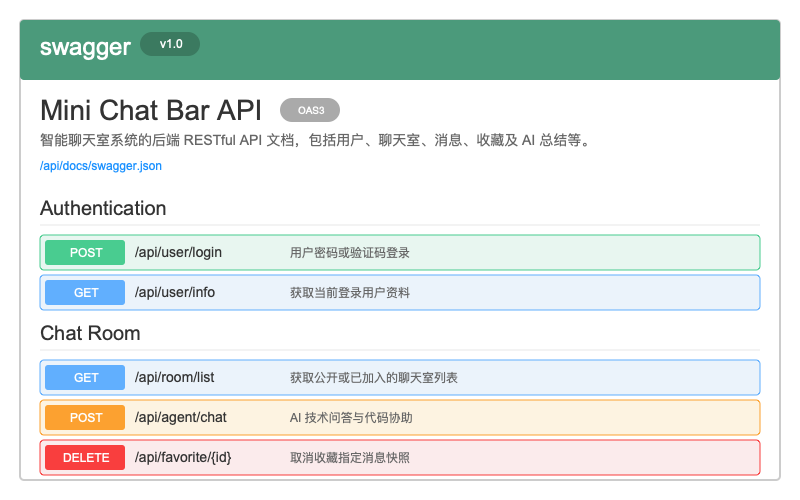
\includegraphics[width=0.88\textwidth,height=0.36\textheight,keepaspectratio]{img/图5_3.png}
\caption{Swagger 接口文档}
\label{fig:5-1}
\end{figure}

后端运行日志能够反映接口进入、Socket 连接和 AI 请求发起等关键状态。将这一部分保留在论文中，有助于更直观地说明系统运行过程中的联调与验证依据。

例如登录接口返回、聊天室消息拉取、Socket 建连和 AI 接口调用，都会在控制台留下时间戳、访问路径和耗时信息，便于联调阶段快速定位问题。

\FloatBarrier

\section{Web前端实现}

前端实现主要集中在 \texttt{ccb/src} 目录下。该部分没有完全按照技术层拆分，而是更接近功能模块划分：登录页、聊天主界面、AI 助手、消息管理和设置页分别对应独立组件或页面。这种组织方式便于围绕具体功能进行维护和定位\cite{vueguide2026,piniadocs2026,electrondocs2026}。

其中，聊天主界面的路由切换逻辑和收藏页的筛选、详情回看逻辑共同构成了前端核心交互。

\subsection{登录/注册页面}

\thesisparenitem{1}{界面功能说明}{登录和注册页面采用翻转卡片形式，正面为登录，背面为注册。登录又分为邮箱密码和邮箱验证码两种方式，卡片底部保留了 Google 和 GitHub 的第三方登录按钮。页面同时提供欢迎信息、输入反馈和登录方式切换，如图~\ref{fig:5-2}和图~\ref{fig:5-3}所示。}

\thesisparenitem{2}{关键交互逻辑}{用户输入邮箱和密码后，前端会先进行格式校验。对于邮箱格式错误、密码为空，或注册时两次密码不一致等情况，页面会在前端阶段直接拦截无效请求。验证码登录额外包含冷却时间控制，60 秒内不能重复获取验证码。登录成功后，页面不仅保存 token，还会继续调用 \texttt{waitForSocketConnection()}，在 Socket 成功连接后发出 \texttt{login} 和 \texttt{user-online} 事件，以完成在线状态初始化。}

\thesisparenitem{3}{与后端的接口交互说明}{邮箱密码登录调用 \texttt{/api/user/\allowbreak login-email}，验证码登录调用 \texttt{/api/user/\allowbreak login-code}，发送验证码调用 \texttt{/api/user/\allowbreak send-verification}，注册调用 \texttt{/api/user/\allowbreak register-email}，第三方登录则直接跳转到 \texttt{/auth/\allowbreak google} 和 \texttt{/auth/\allowbreak github}。}

\thesisparenitem{4}{操作流程}{用户先进入登录页，选择密码登录、验证码登录或第三方登录；若采用本地登录，则输入表单并提交；后端验证通过后返回 token 和用户资料；前端随后保存登录信息、初始化在线状态和 Socket 连接，最后跳转到聊天主界面。}

\begin{figure}[H]
\centering
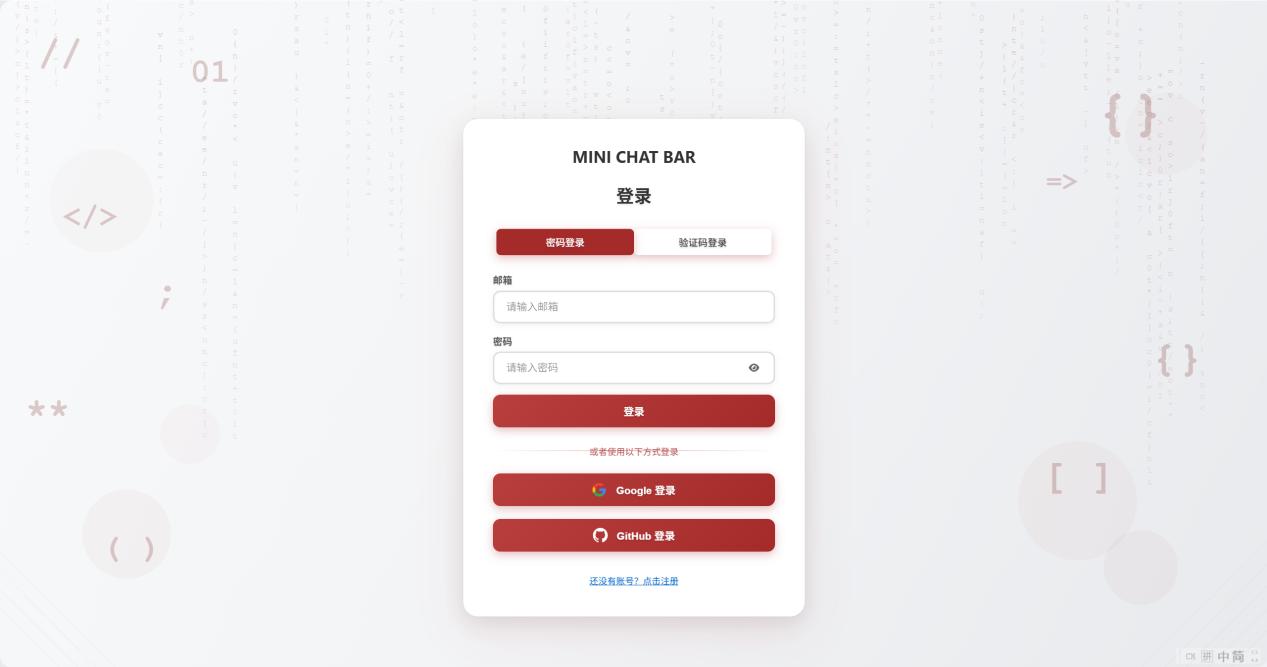
\includegraphics[width=0.88\textwidth,height=0.36\textheight,keepaspectratio]{img/图5_4.png}
\caption{登录页面展示}
\label{fig:5-2}
\end{figure}

\begin{figure}[H]
\centering
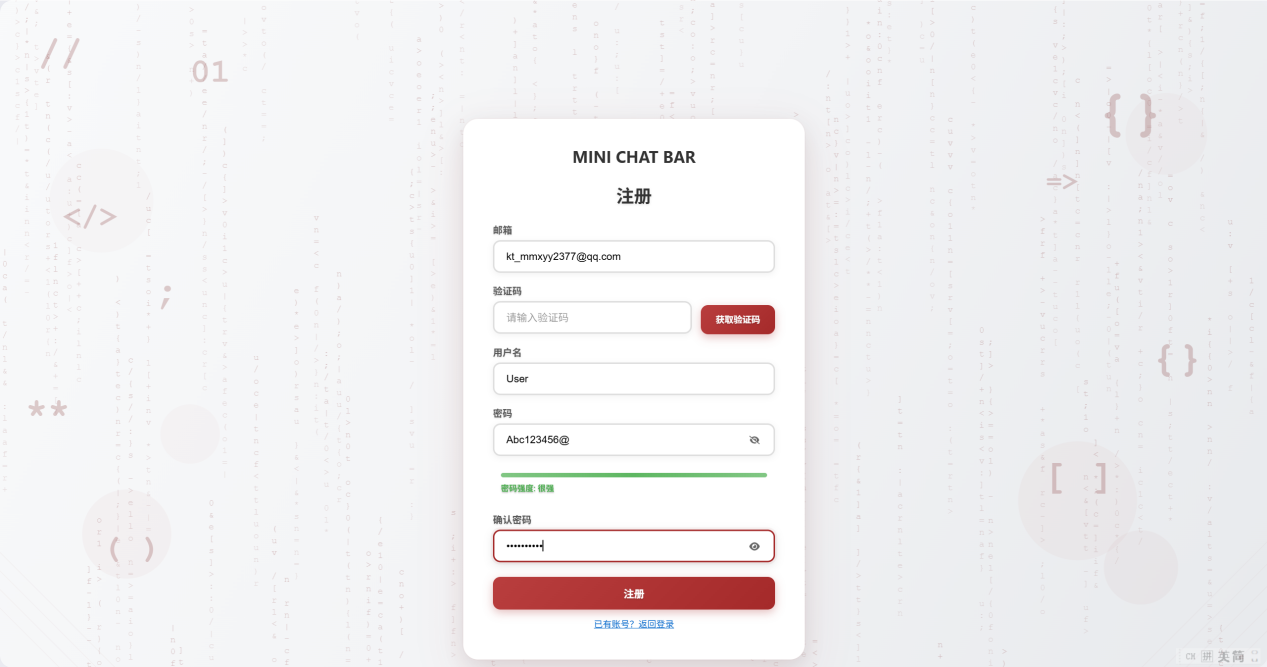
\includegraphics[width=0.88\textwidth,height=0.36\textheight,keepaspectratio]{img/图5_5.png}
\caption{注册页面与表单交互展示}
\label{fig:5-3}
\end{figure}

\FloatBarrier

\subsection{聊天主界面}

\thesisparenitem{1}{界面功能说明}{桌面端采用三栏布局，左侧为导航入口，中间为会话或联系人列表，右侧为详情区；移动端则切换为底部导航形式。该页面主要承担路由组织和区域切换职责，根据当前路由和用户操作决定中间栏与右侧区域的显示内容。主界面总览如图~\ref{fig:5-5}所示，通讯录和聊天室入口分别如图~\ref{fig:5-6}、图~\ref{fig:5-7}所示。}

这一部分对应的前端路由切换与界面组织逻辑见附录G。

\thesisparenitem{2}{关键交互逻辑}{页面初始化时，前端会先检查登录状态，再根据当前路由决定默认展示聊天列表、联系人列表或聊天室列表。用户点击左侧导航栏或底部导航时，页面通过路由切换对应内容区域，而不是仅在界面层隐藏某一块 DOM。用户进入具体联系人或房间后，\texttt{showdetail()} 展示详情函数会将当前目标 ID 写入 \texttt{useChatStore}，并同步传递昵称、头像和聊天类型等参数，为后续消息加载与状态同步提供上下文。}

\thesisparenitem{3}{与后端的接口交互说明}{主界面本身不直接发送消息，但会触发好友列表、群列表、聊天室列表以及用户信息等接口的请求。常见调用包括 \texttt{/api/user/info}、\texttt{/api/user/friends}、\texttt{/room/list} 和 \texttt{/room/chatrooms}。}

\thesisparenitem{4}{操作流程}{用户登录进入主界面后，前端先加载基础资料和列表数据；再根据当前需求切到聊天、联系人或聊天室；选择具体会话后，前端写入当前会话上下文并跳转详情页；详情页继续拉取消息记录并建立需要的 Socket 监听。}

\begin{figure}[H]
\centering
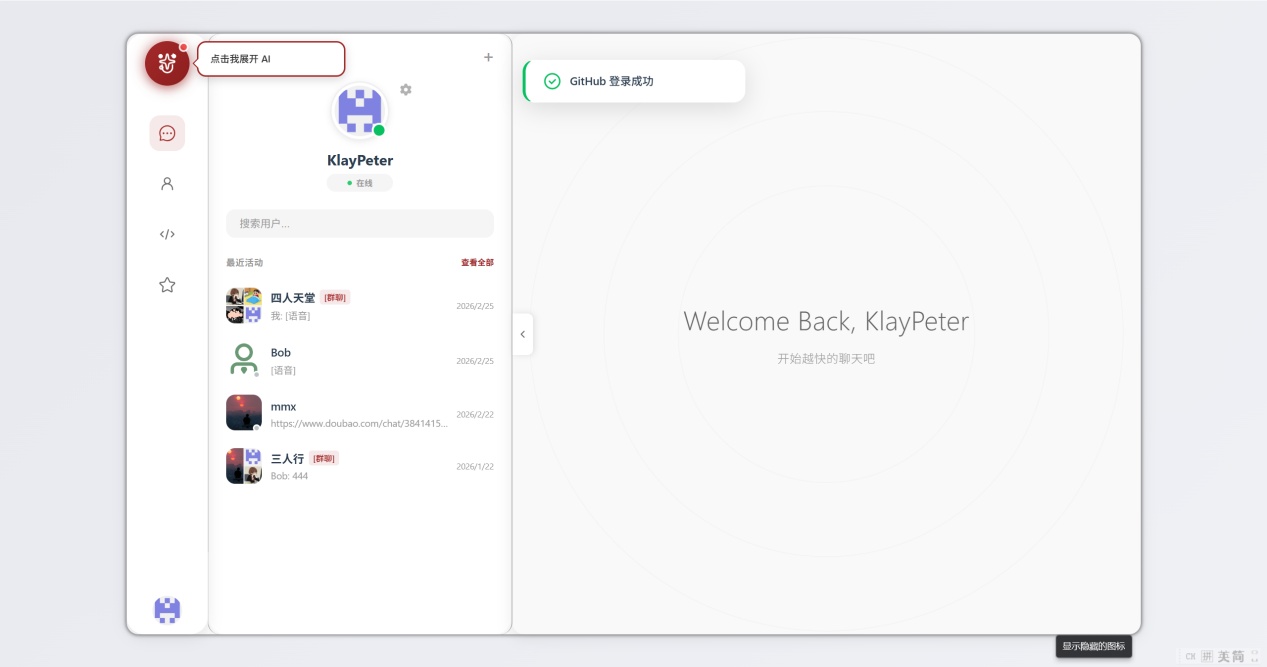
\includegraphics[width=0.88\textwidth,height=0.36\textheight,keepaspectratio]{img/图5_7.png}
\caption{聊天主界面总览}
\label{fig:5-5}
\end{figure}

\begin{figure}[H]
\centering
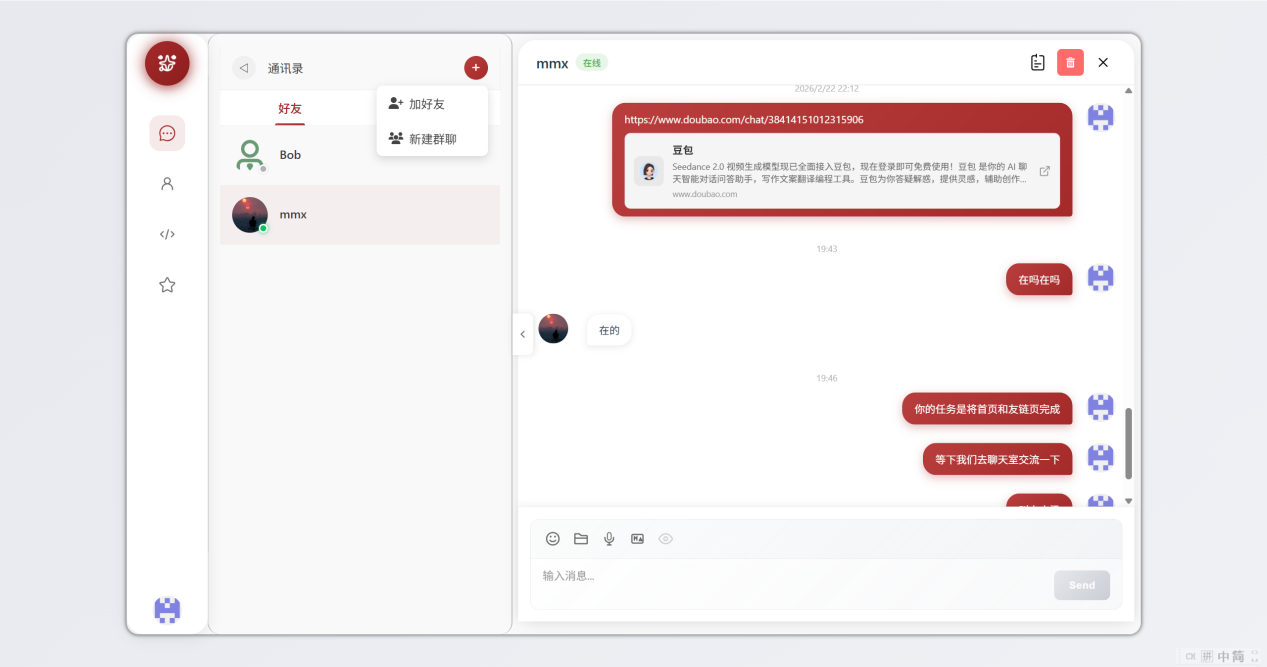
\includegraphics[width=0.88\textwidth,height=0.36\textheight,keepaspectratio]{img/图5_8.png}
\caption{通讯录列表界面展示}
\label{fig:5-6}
\end{figure}

\begin{figure}[H]
\centering
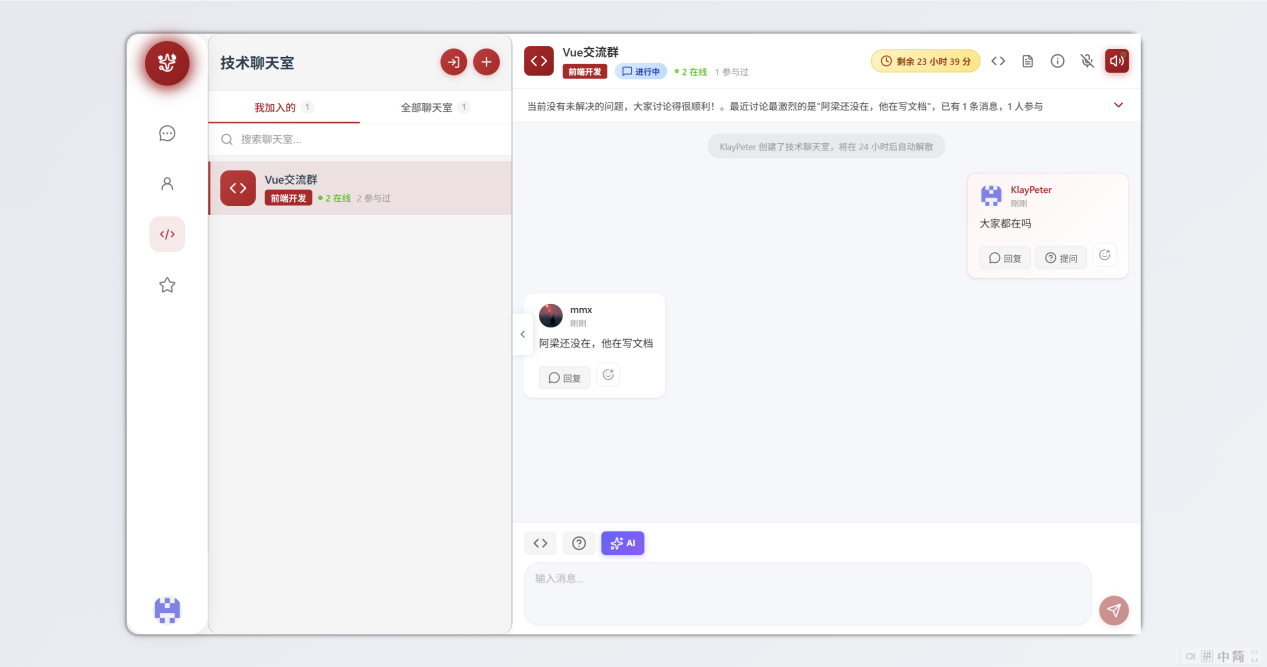
\includegraphics[width=0.88\textwidth,height=0.36\textheight,keepaspectratio]{img/图5_9.png}
\caption{聊天室列表界面展示}
\label{fig:5-7}
\end{figure}

\FloatBarrier

\subsection{AI对话界面}

\thesisparenitem{1}{界面功能说明}{AI 对话相关的界面有两种典型形态。第一种是侧边栏 AI 助手，适合做单独问答、补充解释和上下文延续；第二种是聊天室里的 \texttt{@AI} 交互，它把 AI 回答直接放回房间消息流，更适合多人讨论时一起参考。侧边栏 AI 助手界面如图~\ref{fig:5-9}所示，聊天室中的 AI 回答效果如图~\ref{fig:5-10}所示。}

\thesisparenitem{2}{关键交互逻辑}{侧边栏模式下，用户输入的问题会先追加到本地消息数组，再调用 \texttt{/api/agent/chat} 请求答案，请求成功后再把 AI 回复和来源信息追加到界面。聊天室模式则更强调实时感。用户在输入框里直接输入 \texttt{@AI} 开头的问题，前端会先把原问题发进房间，再触发 \texttt{/api/chatroom-ai/ask-stream}，然后一边接收流式内容，一边刷新当前房间的消息列表。因为后端会把 AI 输出同步广播到房间，所以这个回答不是只对提问者可见，而是房间成员都能看到。}

\thesisparenitem{3}{与后端的接口交互说明}{侧边栏模式主要依赖智能问答和解释接口，聊天室模式则围绕流式问答、智能提示和主动答题几类接口展开。}

\thesisparenitem{4}{操作流程}{AI 模块的操作流程可以概括为：用户打开 AI 面板或在聊天室中输入 \texttt{@AI}；前端提交问题并附带当前上下文；后端结合最近消息和历史检索结果生成回答；回答返回后，前端再按普通消息或流式消息渲染出来。}

\begin{figure}[H]
\centering
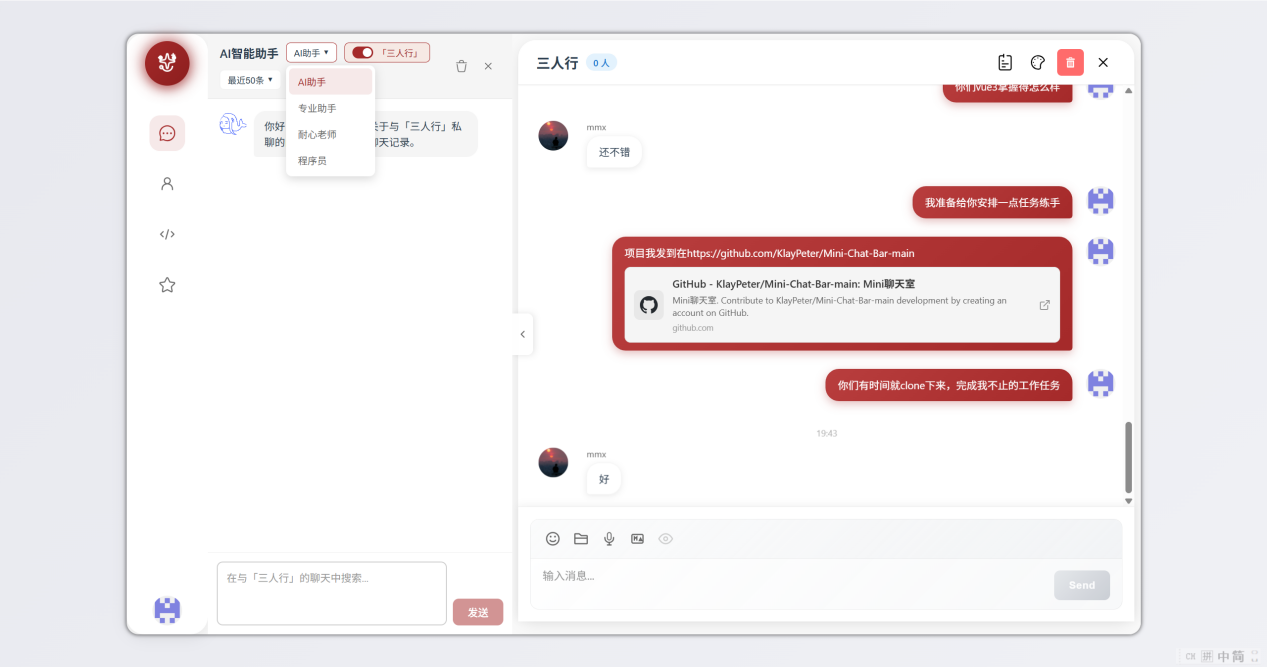
\includegraphics[width=0.88\textwidth,height=0.36\textheight,keepaspectratio]{img/图5_11.png}
\caption{侧边栏 AI 助手界面}
\label{fig:5-9}
\end{figure}

\begin{figure}[H]
\centering
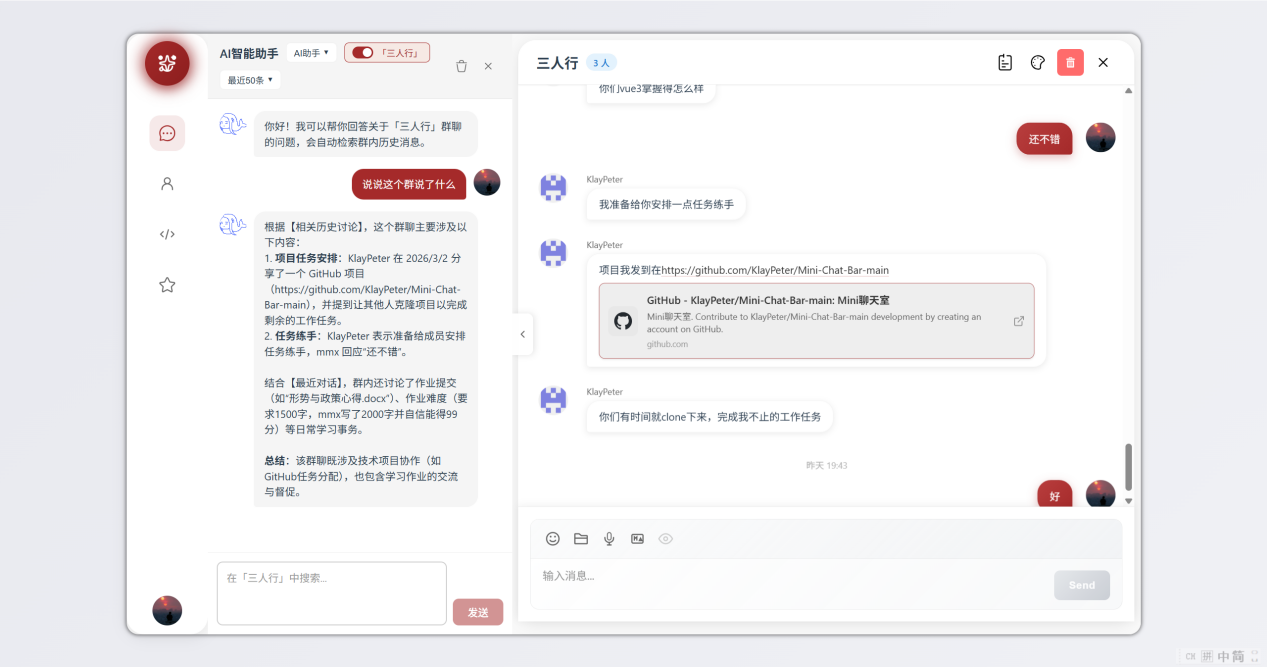
\includegraphics[width=0.88\textwidth,height=0.36\textheight,keepaspectratio]{img/图5_12.png}
\caption{AI 根据历史记录检索后的回答展示}
\label{fig:5-10}
\end{figure}

\FloatBarrier

\subsection{消息列表与会话管理}

\thesisparenitem{1}{界面功能说明}{该部分不仅展示消息列表，还负责最近会话排序、未读数显示、历史消息搜索、收藏整理以及消息转发、撤回等行为。最近会话列表和消息页结合后的效果如图~\ref{fig:5-12}所示，历史消息搜索和收藏页分别如图~\ref{fig:5-13}、图~\ref{fig:5-14}所示。}

\thesisparenitem{2}{关键交互逻辑}{会话列表加载时，前端会先读取好友列表，再查询每个联系人和群聊的最后一条消息及未读数，并按时间重新排序。当前会话打开后，页面继续加载完整历史记录，并按消息类型进行分类渲染。用户点击搜索图标时，前端会在当前消息数组中进行关键词匹配并高亮结果；点击收藏时，则将消息 ID、消息类型和会话 ID 一并发送给后端，以便后续在收藏页单独回看。}

\thesisparenitem{3}{与后端的接口交互说明}{该部分会频繁调用 \texttt{/api/chat/\allowbreak last\_message/\allowbreak :id}、\texttt{/api/chat/\allowbreak unread}、\texttt{/api/chat/\allowbreak messages/\allowbreak :id} 等消息接口，以及 \texttt{/room/\allowbreak :roomId/\allowbreak messages}、\texttt{/api/\allowbreak favorites} 和 \texttt{/api/\allowbreak favorites/\allowbreak :messageId} 等房间与收藏接口。}

\thesisparenitem{4}{操作流程}{消息列表与会话管理的基本流程是：先加载会话摘要信息，再根据用户选择打开具体会话；进入会话后加载完整历史消息；如果用户执行搜索、收藏或删除等操作，再分别调用对应接口更新状态，并同步刷新列表（相关实现见附录H）。}

\begin{figure}[H]
\centering
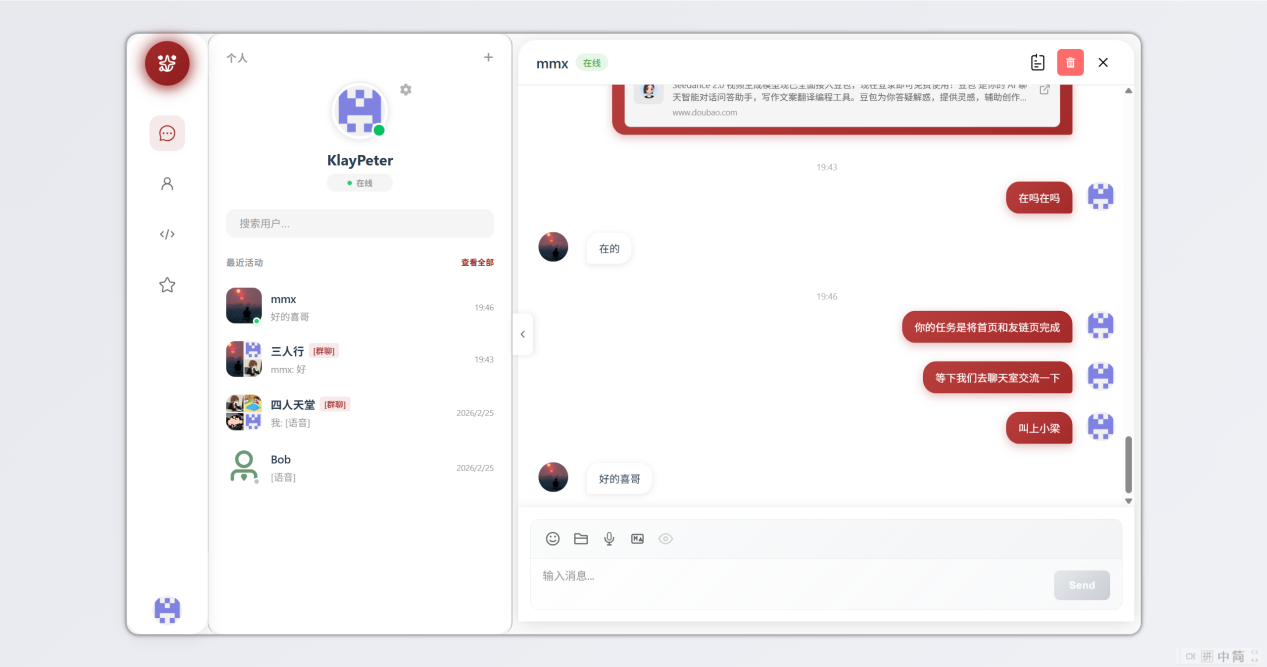
\includegraphics[width=0.88\textwidth,height=0.36\textheight,keepaspectratio]{img/图5_14.png}
\caption{会话列表与私聊界面展示}
\label{fig:5-12}
\end{figure}

\begin{figure}[H]
\centering
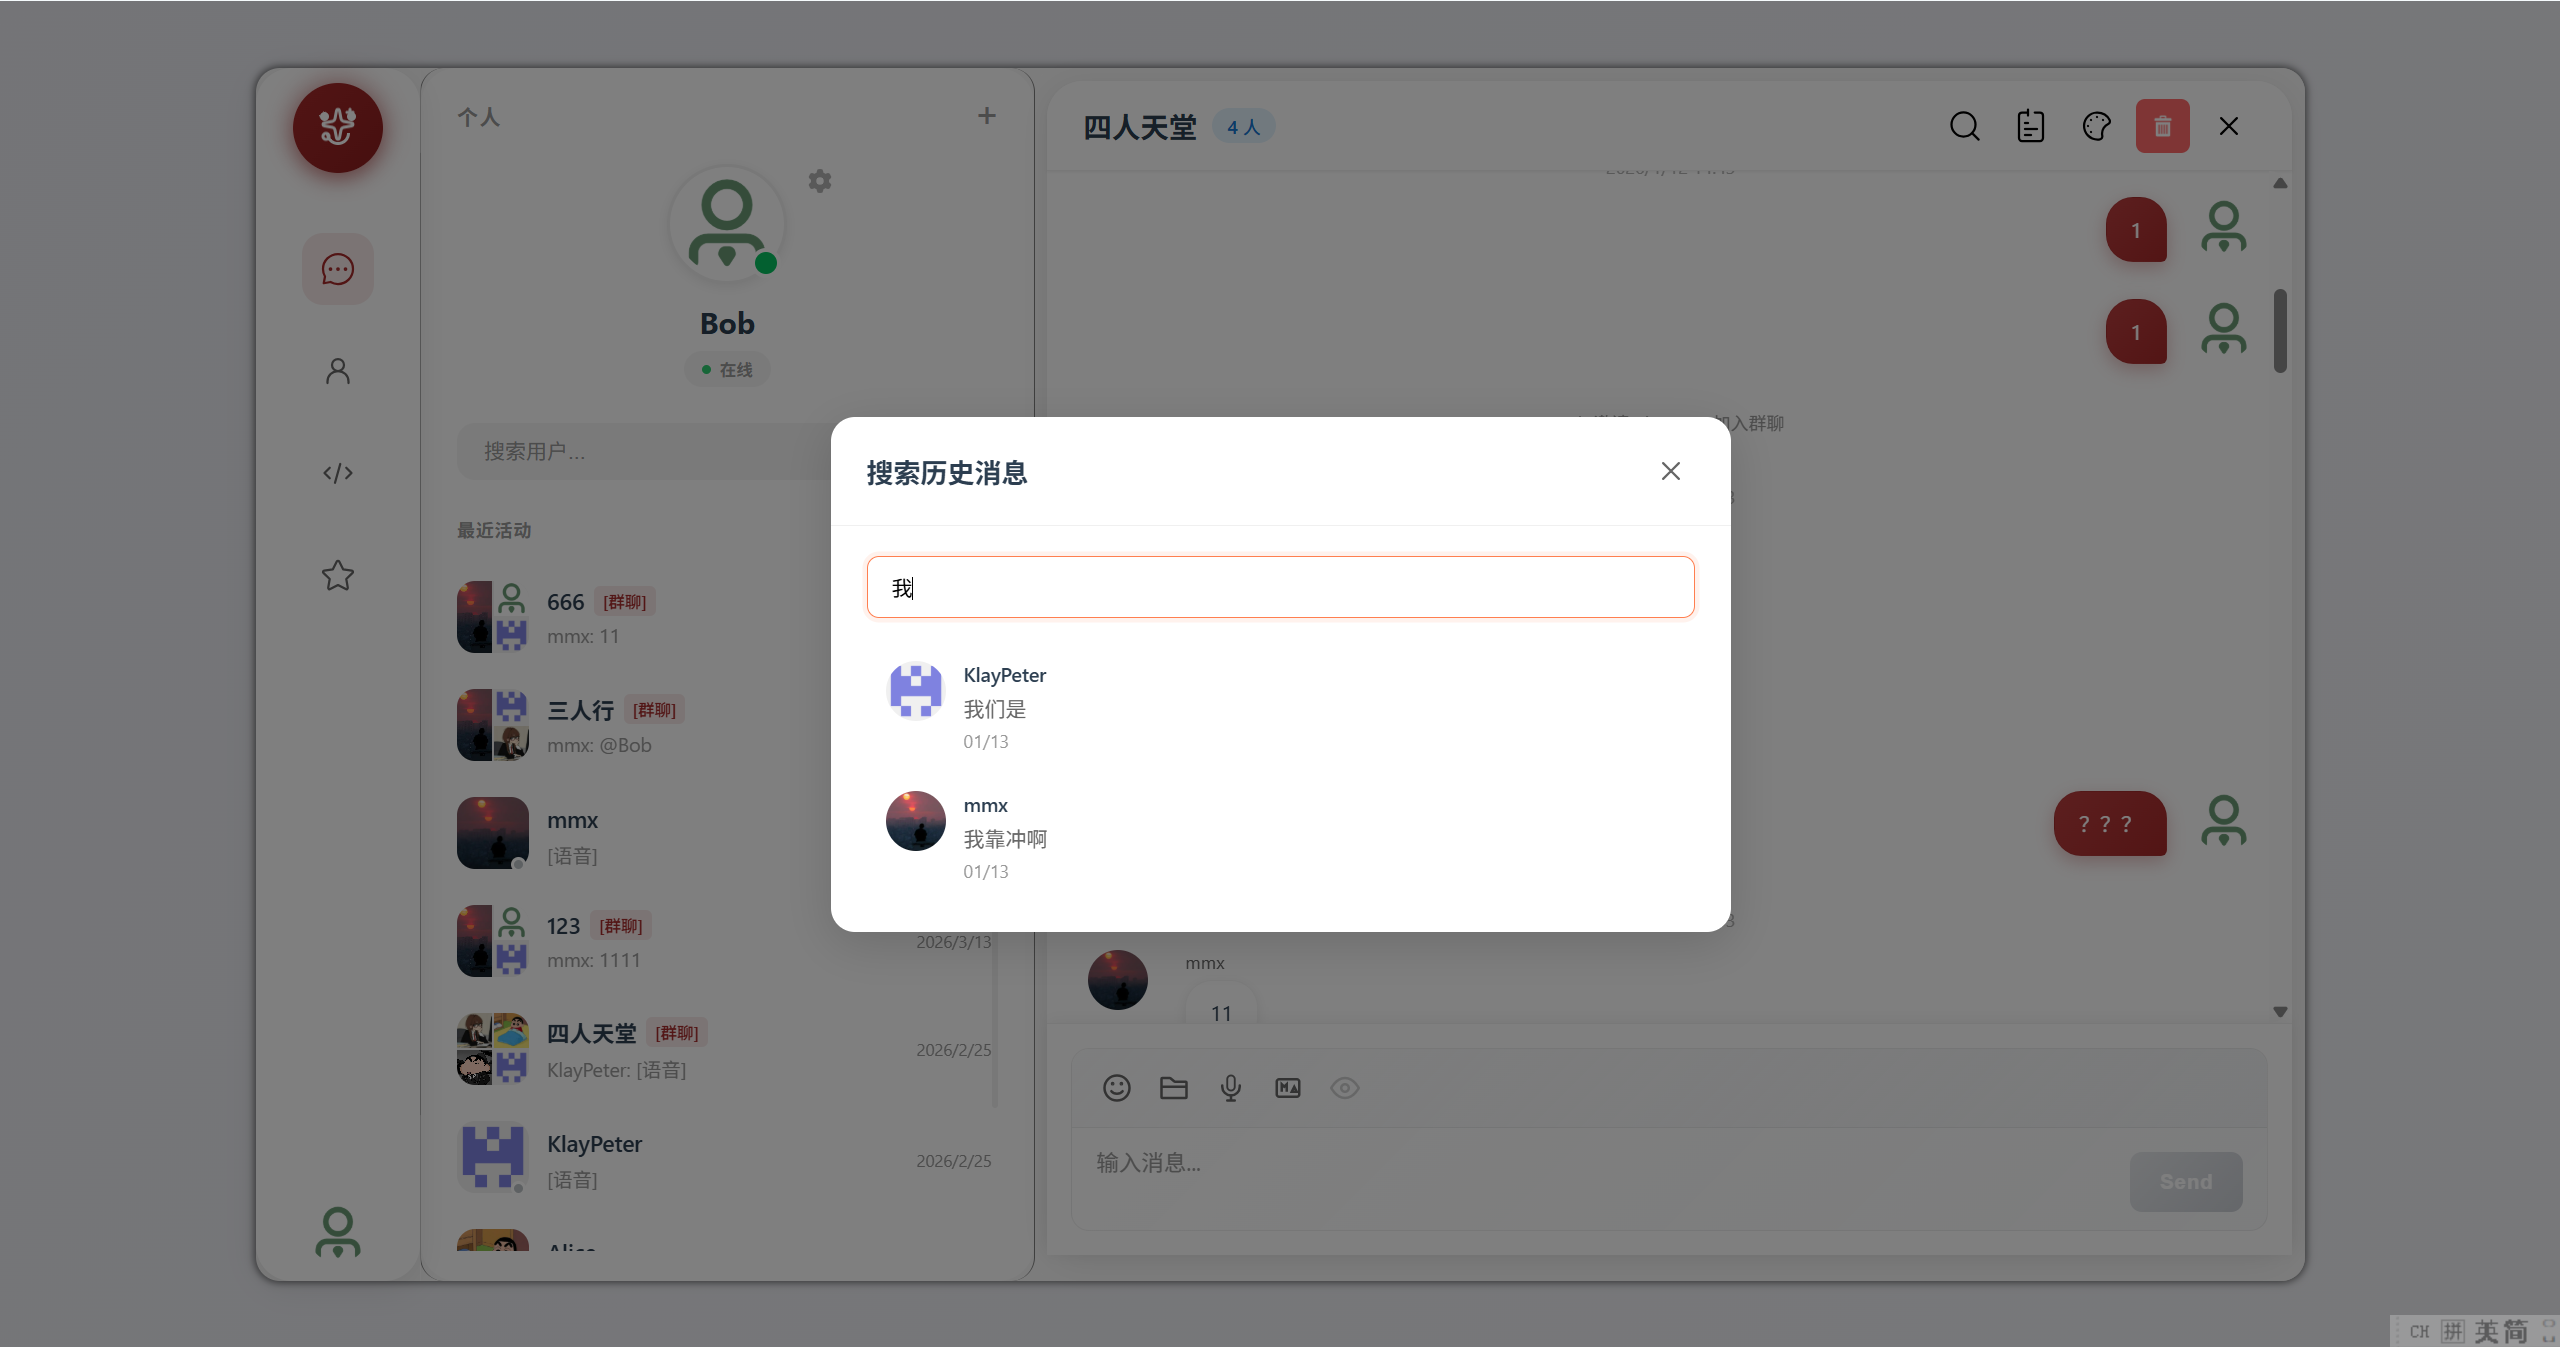
\includegraphics[width=0.88\textwidth,height=0.36\textheight,keepaspectratio]{img/图5_15.png}
\caption{历史消息搜索界面展示}
\label{fig:5-13}
\end{figure}

\begin{figure}[H]
\centering
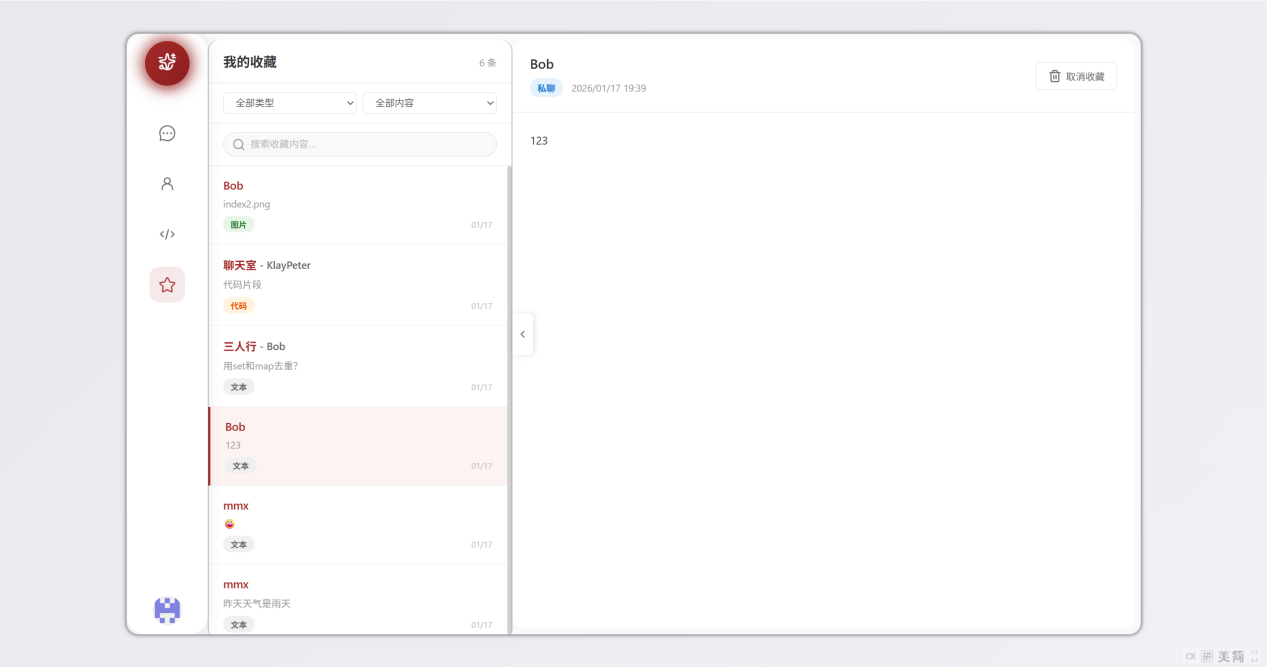
\includegraphics[width=0.88\textwidth,height=0.36\textheight,keepaspectratio]{img/图5_16.png}
\caption{收藏页面展示}
\label{fig:5-14}
\end{figure}

\FloatBarrier

\subsection{设置与个人中心}

\thesisparenitem{1}{界面功能说明}{设置与个人中心包含头像上传、预设头像切换、用户名修改、主题切换和退出登录等功能。该模块虽然不像聊天页那样集中承载消息交互，但与主界面的资料展示保持联动。用户更新头像后，最近会话列表、当前聊天页和其他在线用户看到的资料都需要同步刷新。设置与个人中心界面的实际效果如图~\ref{fig:5-16}所示。}

\thesisparenitem{2}{关键交互逻辑}{用户上传头像时，前端先把图片发到 \texttt{/api/upload}，拿到文件地址后再调用 \texttt{/api/user/avatar} 更新资料；修改用户名时，则直接调用 \texttt{/api/user/username}。更新成功后，前端会发出 \texttt{avatar-updated} 事件，通知其他在线用户同步刷新头像。主题切换则通过 \texttt{useThemeStore} 完成，并把主题键值写入 \texttt{localStorage}，这样刷新页面后仍然保留用户上一次的选择。}

\thesisparenitem{3}{与后端的接口交互说明}{头像上传依赖 \texttt{/api/upload}，资料更新依赖 \texttt{/api/user/\allowbreak avatar} 和 \texttt{/api/user/\allowbreak username}，界面刷新时则重新读取 \texttt{/api/user/\allowbreak info}。}

\thesisparenitem{4}{操作流程}{设置模块的基本流程为：用户打开设置弹窗，修改头像、用户名或主题；前端调用对应接口并保存结果；保存成功后，同步刷新本地资料和相关组件；如果修改内容会影响其他在线用户的显示结果，还会继续通过 Socket 广播更新。}

\begin{figure}[H]
\centering
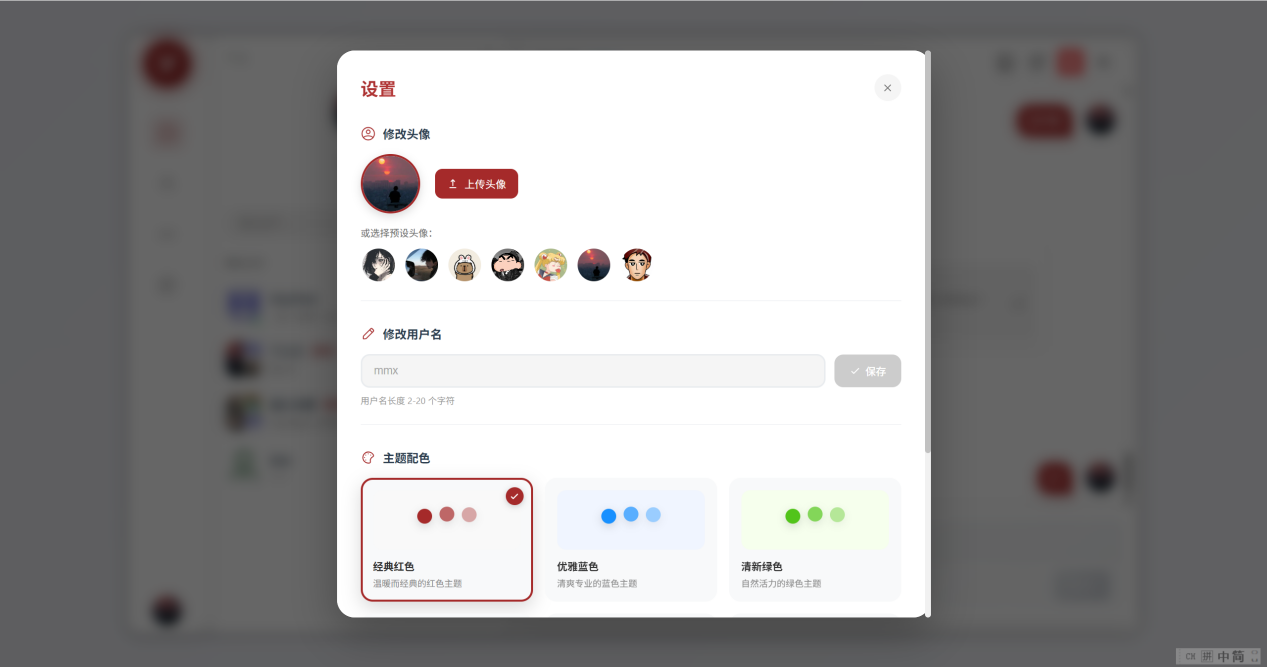
\includegraphics[width=0.88\textwidth,height=0.36\textheight,keepaspectratio]{img/图5_18.png}
\caption{设置与个人中心界面展示}
\label{fig:5-16}
\end{figure}

\FloatBarrier

\subsection{Web端消息流转与状态管理}

从界面表现看，Web 端的核心功能集中在登录、消息收发和会话切换，而这些功能能稳定运行，依赖于底层的消息流转和状态管理。私聊发送时，系统会先调用 \texttt{/api/chat/messages/:id} 将消息写入数据库，再通过 \texttt{private-message} 事件提醒另一端刷新；群聊发送时，前端调用 \texttt{/room/:roomId/messages}，后端控制器保存成功后会主动广播 \texttt{group-message}，因此前端不需要重复发送同名消息。收到消息后，界面再根据 \texttt{messageType} 区分文本、图片、文件、语音和代码等不同渲染分支，从而完成统一消息列表中的分类展示。

WebSocket 的使用也做了分层处理。普通聊天页主要依赖socket提供的全局连接，这一层包含自动重连、断线提示和心跳包；聊天室详情页则额外维护房间级事件，包括 \texttt{join-group}、\texttt{online-count}、\texttt{ai-stream-chunk}、\texttt{join-voice-room} 等。这样一来，普通会话页和聊天室页就能分别承载不同复杂度的实时交互。

状态管理方面，系统虽然使用了 Pinia，但并没有把所有状态都集中到全局 store。全局配置文件只保留 \texttt{currentChatUser} 和按用户区分的消息列表；会话列表、未读数、当前房间详情、搜索结果和收藏状态等内容，仍由各组件内部的 \texttt{ref} 与自定义事件配合维护。比如群聊消息发送后，前端会发出 \texttt{group-message-sent} 事件通知列表刷新；聊天室打开后，再通过 \texttt{group-chat-opened} 事件清除未读数。这样的组织方式和当前项目规模基本匹配。

\FloatBarrier

\section{桌面端实现}

桌面端在界面层仍复用了同一套前端页面，但额外增加了 Electron 封装。因此，它与 Web 端的主要差异不在聊天主流程本身，而在窗口管理、系统托盘、本地通知和 IPC 通信等桌面环境能力。

\subsection{系统托盘功能}

桌面端由 Electron 主进程统一管理窗口和托盘行为。程序启动后会先创建主窗口，再创建托盘图标。在 Windows 下，用户关闭主窗口时，程序不会直接退出，而是隐藏到系统托盘继续运行。托盘左键用于显示或隐藏主窗口，右键菜单提供“打开应用”和“退出应用”两个入口，这样桌面端就能在后台继续接收消息。

托盘点击事件会在“显示主窗口”和“隐藏到后台”之间切换，保证程序关闭窗口后仍可保持驻留状态和未读提醒能力。

桌面端在收到新消息后的未读提醒和任务栏反馈效果如图~\ref{fig:5-18}所示。这个设计是在复用网页界面的基础上，补充桌面环境下的消息提醒机制。

\begin{figure}[H]
\centering

\includegraphics[width=0.88\textwidth,height=0.36\textheight,keepaspectratio]{img/图5_20.png}
\caption{桌面端未读提醒展示}
\label{fig:5-18}
\end{figure}

\FloatBarrier

\subsection{本地通知}

本地通知由消息提醒管理模块、预加载脚本和 Electron 主进程三部分配合完成。渲染进程收到新消息后，会通过 \texttt{window.electronAPI.notifyNewMessage()} 把未读数发给主进程；主进程根据平台再去设置任务栏闪烁、Overlay 图标、托盘提示和最近消息预览。用户如果从托盘预览里点击某个会话，主进程还会继续把 \texttt{open-chat} 事件发回渲染进程，前端再切到对应私聊或群聊。

渲染进程把未读数和最近消息通过 \texttt{electronAPI} 发送给主进程后，主进程再统一负责闪烁提醒、角标更新和托盘预览，从而把桌面通知逻辑和业务页面分开处理（相关实现见附录I）。

系统托盘的图标、菜单入口与后台驻留形态如图~\ref{fig:5-19}所示。托盘机制使桌面端在关闭主窗口后仍能继续接收消息，并保留快速唤起入口。

\begin{figure}[H]
\centering
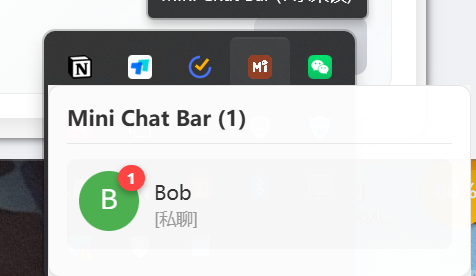
\includegraphics[width=0.88\textwidth,height=0.36\textheight,keepaspectratio]{img/图5_21.png}
\caption{系统托盘展示}
\label{fig:5-19}
\end{figure}

\FloatBarrier

\subsection{与后端和WebSocket通信}

桌面端和后端通信的基础方式并没有变化，仍然由 Axios 调用 REST 接口，并由 Socket.IO 负责实时同步。区别在于，桌面端比 Web 端多了一层由通信转接层暴露的 \texttt{electronAPI}，使渲染进程在不直接接触 Node API 的前提下，也能将“新消息提醒”“清空角标”“打开对应会话”等动作交给主进程处理。

从这一点看，桌面端并不是另一套独立业务系统，而是在 Web 端原有聊天逻辑之外补充桌面环境能力。这样可以保持核心业务代码只维护一份，由桌面端单独处理托盘、通知和窗口行为，从而减少后续功能更新时与 Web 端的实现分叉。
